% Chapter 3

\chapter{Belize Expedition} % Main chapter title

\label{Chapter3}

%-------------------------------------------------------------------------------
%-------------------------------------------------------------------------------
\begin{figure}[ht]
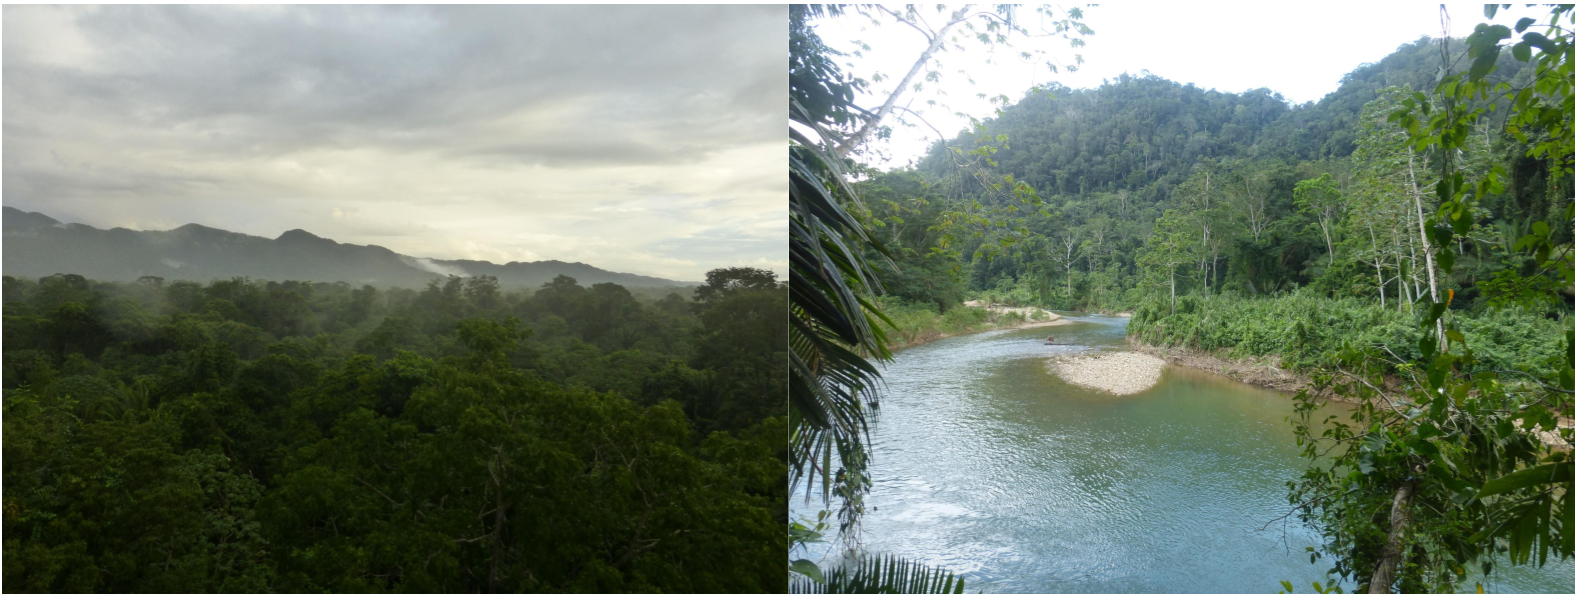
\includegraphics[width=0.9\textwidth]{Figures/TripPhotos.png}
\caption{Photos taken during the expedition to the Bladen National Reserve}
\label{fig:TripPhotos}
\end{figure}

\section{Study Sites}

We collected aerial survey data over two adjacent protected areas located in the Maya Mountains in the Toledo District of southern Belize ~\ref{fig:BFREE-Map}. The first was a 467-hectare (1,153-acre) private protected reserve administered by the Belize Foundation for Research and Environmental Education (BFREE; 16.5 N, 88.6 W).  The second site was a 170-hectare (420-acre) valley within the 39,270-hectare (97,039-acre) Bladen Nature Reserve (BNR), a national park-like, government reserve (Forestry Department, Government of Belize).  The two sites are part of the 607,028 hectares (1.5 million acres) Maya Mountains protected area system, often considered one of the largest remaining unspoiled, mixed tropical forest ecosystems remaining in Central America \cite{Brewer}, \cite{Olivet}, \cite{Dourson}.  Elevation and precipitation in the Maya Mountains range from 80 to 1000 meters with rainfall averages between 2500 and 3000 millimeters (80-100 inches) of rain per year. The area has distinct wet and dry seasons, of which $89\%$ of the rainfall occurs between May and December \cite{Brokaw}.  Both the BFREE and BNR areas have been classified with only coarse-scale, generalized habitat categories including: mainly tall and low tropical evergreen forest (low forest is referred to as “Broken Ridge” in Belize), and a variety of disturbed habitats including early secondary forest, riparian edge, seasonally inundated forests, and Cacao agroforest at BFREE; and tall to medium, tropical evergreen forests as well as smaller amounts of mixed low forest with some disturbed riparian edge near the Bladen River for the BNR.

For this we work we split these areas into three separate entities. First is BFREE area discussed above. Second is Oro which is a smaller valley that required to fly past BFREE along a river. Third is Ramos which required flying a considerable distance along a river before reaching a small open valley.

\begin{figure}[ht]
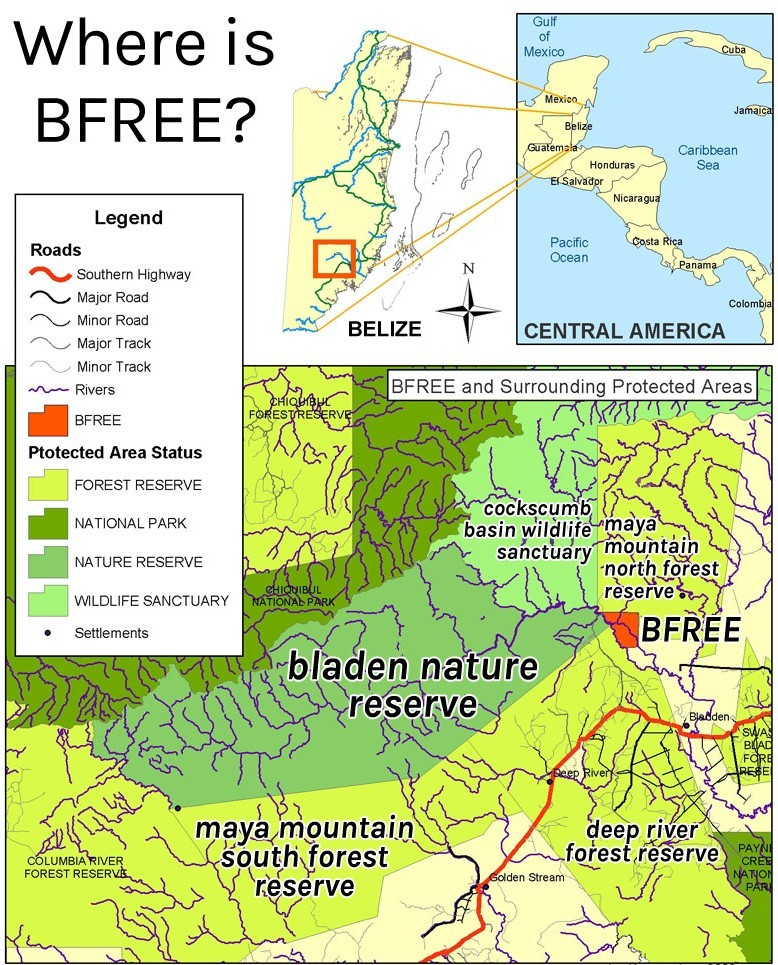
\includegraphics[width=0.4\textwidth]{Figures/BFREE-Map.jpg}
\caption{Map of Bladen Nature Reserve and BFREE site}
\label{fig:BFREE-Map}
\end{figure}

\section{Flight System}

The imagery was collected using a 2-meter wingspan, fixed-wing airplane-type UAV, model Volantex Ranger EX  ~\ref{fig:Volantex}. The Ranger was fitted with an Ardupilot autopilot system, which allows for autonomous control over long range flights. This flight system (Ranger + Ardupilot) was selected due to its rugged design, payload capacity, and long range. The tough body and 60 km range were requirements for use in Belize where landing areas were rough on the airframe. Flight paths were pre-planned in QGround Control Station, an open source ground control station software. All flights were conducted with a Sony QX1 for visible imagery, and a modified Canon S100 for near infrared, which limited vehicle range due to weight, but lowered the number of required flights. The cameras were triggered externally by the autopilot system based on distance flown. A bill of materials is given in table ~\ref{table:FlightBOM}. Collecting the same data using a manned flight system would be orders of magnitude more expensive.


\begin{table}[]
\centering
\caption{My caption}\label{table:FlightBOM}
\label{my-label}
\begin{tabular}{ll}
Item                                                    & Cost                          \\ \hline
ranger airframe                   & \$140.00 \\
ranger servos                     & \$150.00 \\
ranger power system (esc + motor) & \$150.00 \\
ranger telemetry kit              & \$200.00 \\
ranger rc                                               & \$40.00                       \\
3dr pixhawk                                             & \$200.00                      \\
pixhawk airspeed                                        & \$55.00                       \\
pixhawk gps/compass                                     & \$80.00                       \\
frsky taranis rc tx                                     & \$240.00                      \\
batteries                                               & \$500.00                      \\
gcs laptop                                              & \$200.00                      \\
chargers                                                & \$280.00                      \\
Sony QX1 + 20mm lens                                    & \$750.00                      \\
NGB Converted Canon S100                                & \$600.00                      \\ \hline
Total                                                   & \$3585
\end{tabular}
\end{table}

\begin{figure}[ht]
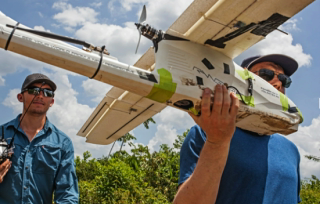
\includegraphics[width=0.6\textwidth]{Figures/Volantex.png}
\caption{Volantex Ranger Ex about to be hand launched for its last day of data collection. The platform is easily managed by a team of two people and can be launched without out external equipment making it an ideal platform for difficult to access areas.}
\label{fig:Volantex}
\end{figure}

\section{Flights}

Data was collected over three days over a total of six flights. The paths of all flights are shown in ~\ref{fig:FlightPaths}. All flights began from the same location on a dirt road in a corn field adjacent to the rainforest allowing for ample room for takeoff and landing. One of the downsides to commercial MAVs is that generally speaking they are not water proof nor very water resistant. Rainforests often have unpredictable weather patterns that interfere with flights. During this trip we were forced to cut several flights shorter than we desired.

\begin{figure}[ht]
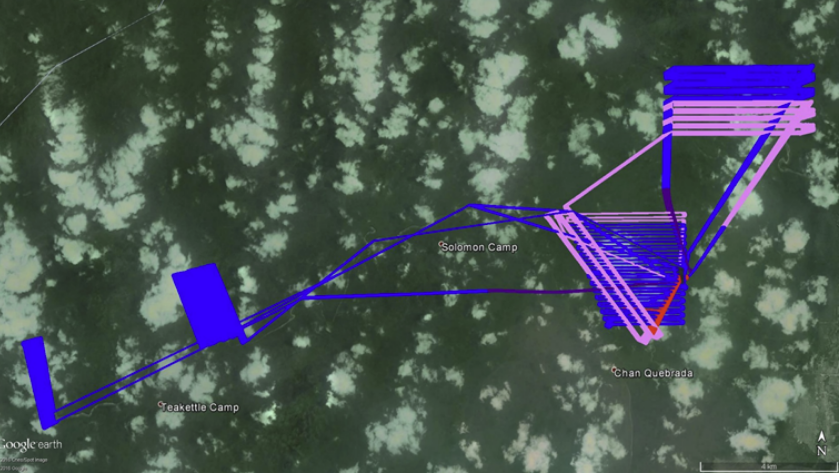
\includegraphics[width=0.8\textwidth]{Figures/FlightPaths.png}
\caption{Flight Paths Over BFREE, Oro and Ramos Survey Sites}
\label{fig:FlightPaths}
\end{figure}

\section{Post Processing}

\begin{figure}[ht]
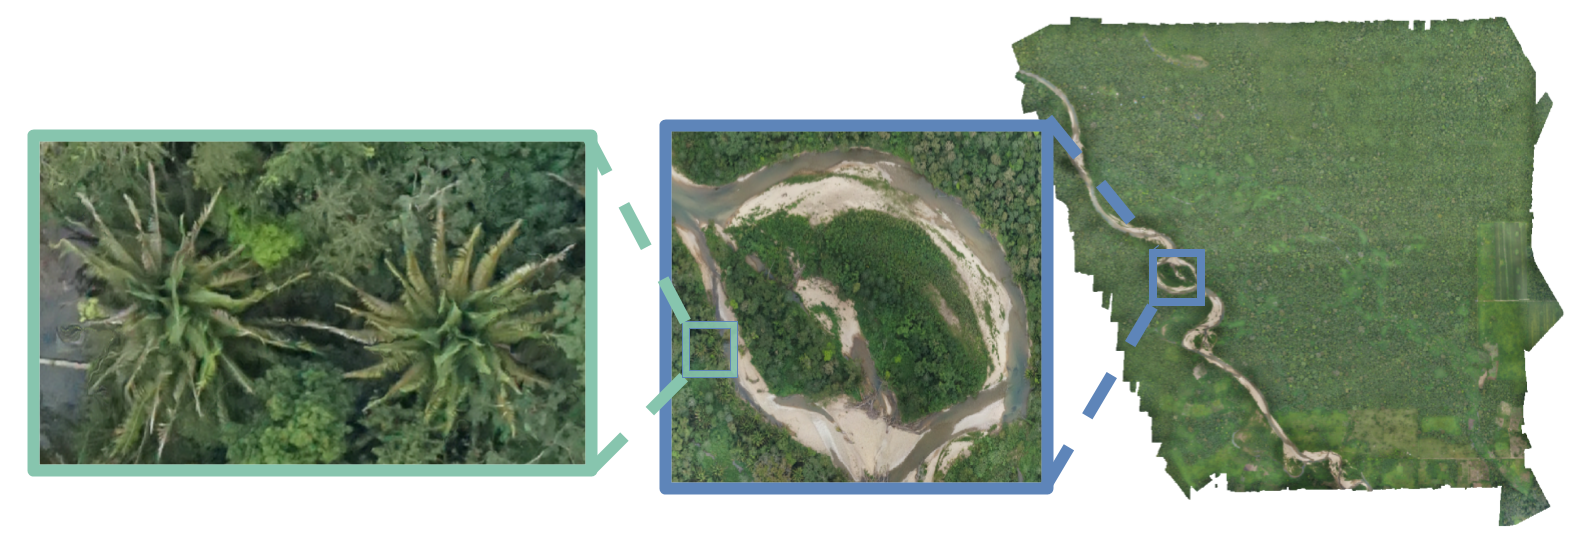
\includegraphics[width=0.8\textwidth]{Figures/Orthomosaic.png}
\caption{Orthomosaic of our main test site BFREE. An example of zooming down on the two palm trees is shown to demonstrate the resolution of the orthomosaic. The size of the orthomosaic is 16GB.}
\label{fig:Orthomosaic}
\end{figure}

The flight paths were designed to collect enough overlapping images to recreate the canopy in 3D and generate orthorectified mosaics through the process of SfM using Agisoft Photoscan Professional version 1.2.6. We produced three separate TIFs for the area: a RGB orthomosaic, a NIR orthomosaic, and a digital elevation map (DEM). The BFREE main survey site is a wide open with very little terrain. The lack of elevation changes allowed the UAV to safely fly at lower altitudes and collect higher resolution data. The resolution for the BFREE site is 4.93 cm/pixel covering a $8.73km^2$ site. The other two sites: Ramos and Oro lay along a river that cut through mountainous terrain which forced the UAV to fly at higher altitudes to maintain a safe boundary. The Ramos and Oro flights have nearly half the resolution with at around 10 cm/pixel with $20.50km^2$ and $16.37km^2$ respectively. Additionally these two flights encountered more low hanging fog and poor lighting conditions as can be seen in ~\ref{fig:OroClouds} making the task of classification more difficult. This requires the tree detector to be robust to resolution variations as well as lighting conditions.

\begin{center}
    \begin{table}[h]\footnotesize
        \caption{Post Processing Statistics generated by creating othrorectified mosaics through Agisoft.}\label{table:AgisoftStats}
        \begin{tabular}{| l | l | l | l | l |}
        \hline
        Site & Flying Altitude (m) & Number of Images & Resolution (cm/pixel) & Area ($km^2$) \\ \hline
        BFREE & 248 & 1529 & 4.93 & 8.73 \\
        Oro Main & 535 & 325 & 10.5 & 3.3 \\
        Oro Joiner & 543 & 156 & 10.5 & 2.27 \\
        Oro Path & 594 & 412 & 11.7 & 10.8 \\
        Ramos & 537 & 769 & 10.6 & 20.5 \\
        \hline
        \end{tabular}
    \end{table}
\end{center}

Additionally we used the Agisoft softare to generate orthorectified mosaics. Orthomosaics are similar to the panoramas popular on mobile phone; the basic premise being that by taking and stitching together many images you end up with a single cohesive image that represents an area larger than you could normally capture with a single photograph. Orthomosaics go a step farther by reprojecting the image into a top down view which is called orthorectification. See ~\ref{fig:Orthomosaic} to see the orthorectified image of the BFREE site. This is crucial to obtaining accurate population counts, since at most you want a single instance of a tree to be represented in the data. If we had simply used the raw images we might have had several pictures of the same tree.

Meta-data for each image i.e. GPS location and orientation is captured from the autopilot. This information allows the software to create a correspondence between each pixel in the orthomosaic and a global latitude, longitude. Meaning for each instance of a tree we find we can relate exactly where in the world that tree is located.

\begin{figure}[ht]
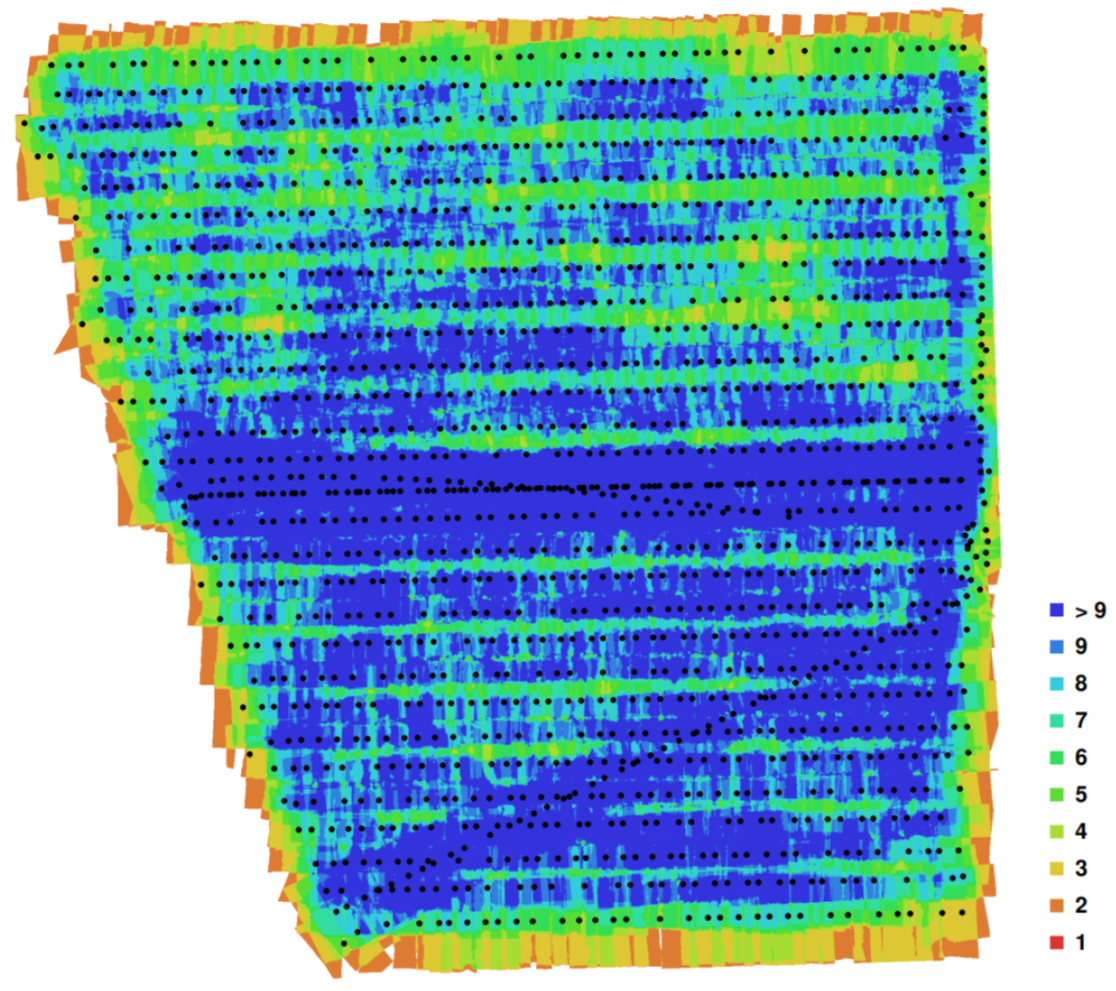
\includegraphics[width=0.8\textwidth]{Figures/BFREE-DEM.png}
\caption{Digital elevation map produced using Agisoft SfM software suite. Color codes represent the number overlapping images for that pixel. This additionally information could be very informative in discriminating between trees. Future research might examine how this information could be included in a CNN architecture.}
\label{fig:BFEE-DEM}
\end{figure}

\begin{figure}[ht]
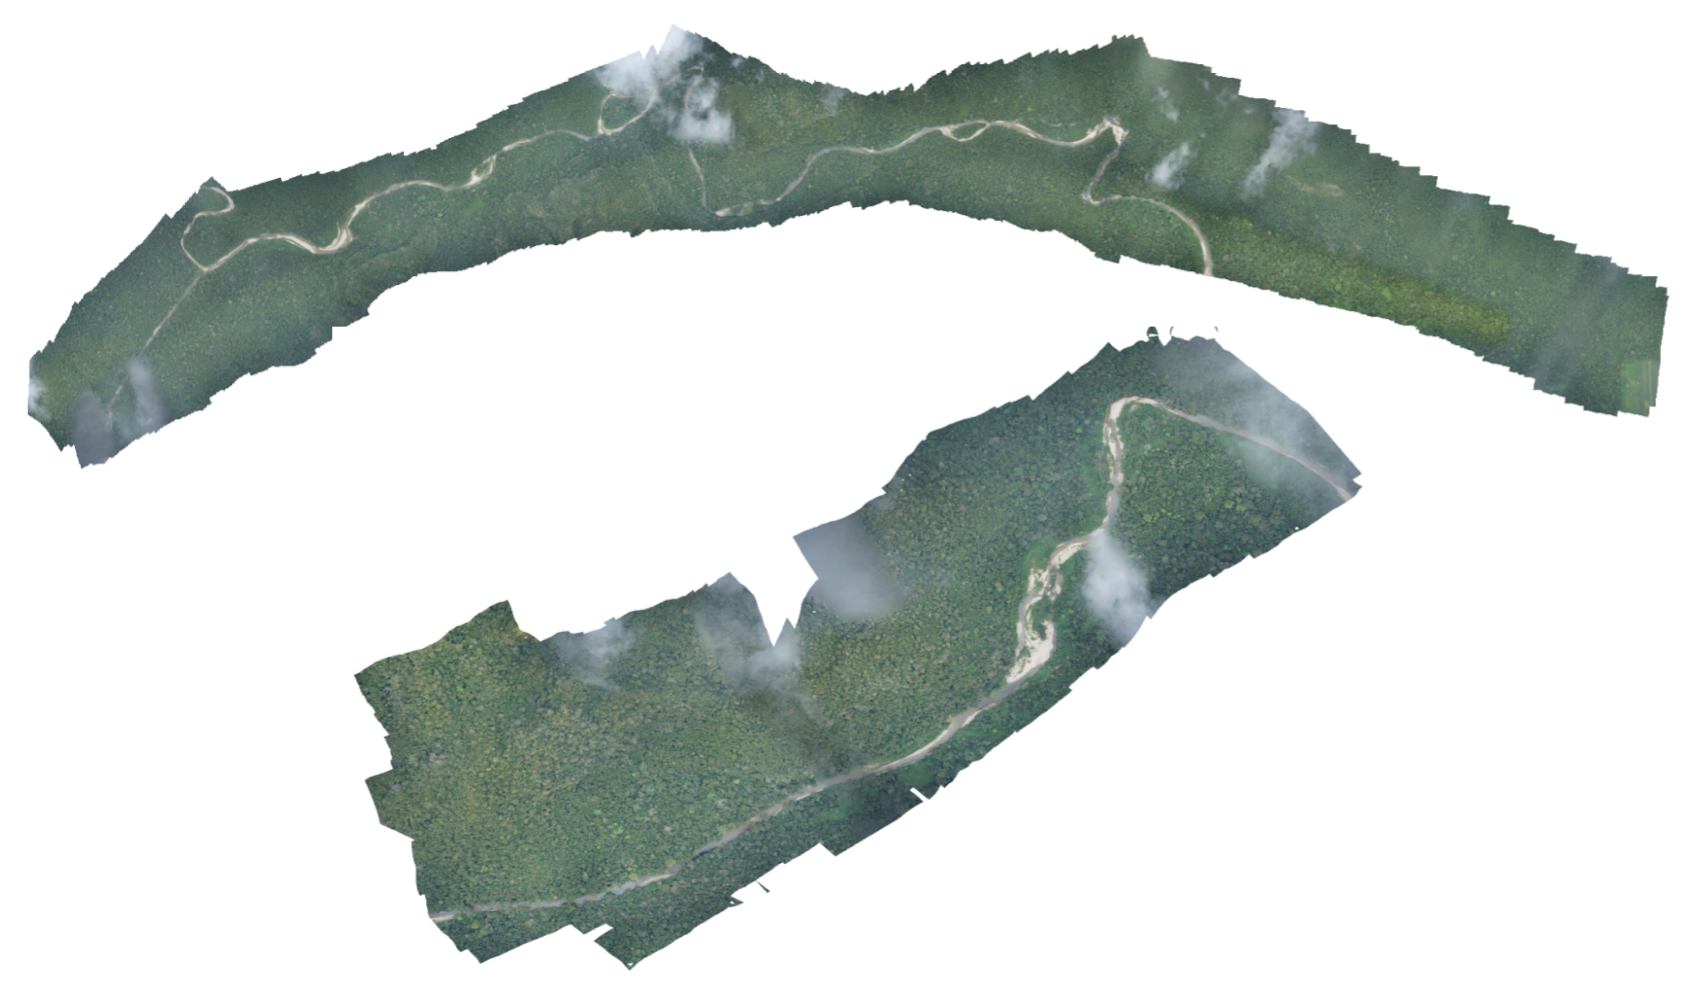
\includegraphics[width=0.8\textwidth]{Figures/OroClouds.png}
\caption{Two separate parts of the Oro site showing low hanging cloud coverage and various lighting conditions.}
\label{fig:OroClouds}
\end{figure}
